\documentclass[12pt]{beamer}
\usepackage[T2A]{fontenc}
\usepackage[utf8]{inputenc}
\usepackage[english]{babel}
\usepackage{amssymb,amsfonts,amsmath,mathtext}
\usepackage{cite,enumerate,float,indentfirst}
\usepackage{longtable,xspace,subcaption}  
\usepackage{amsmath}

\newcommand{\splitline}{\vspace{0.4cm}}
\graphicspath{{images/}}

\usetheme{Singapore}
\usecolortheme{beaver}

\setbeamercolor{footline}{fg=red}
\setbeamertemplate{footline}{
  \leavevmode%
  \hbox{%
  \begin{beamercolorbox}[wd=.333333\paperwidth,ht=2.25ex,dp=1ex,center]{}%
    Innopolis University
  \end{beamercolorbox}%
  \begin{beamercolorbox}[wd=.333333\paperwidth,ht=2.25ex,dp=1ex,center]{}%
    CloSpan
  \end{beamercolorbox}%
  \begin{beamercolorbox}[wd=.333333\paperwidth,ht=2.25ex,dp=1ex,right]{}%
  page \insertframenumber{} of \inserttotalframenumber \hspace*{2ex}
  \end{beamercolorbox}}%
  \vskip0pt%
}
\fontsize{9}{10}\selectfont
\newcommand\fontvi{\fontsize{10}{12}\selectfont}
\newcommand{\itemi}{\item[\checkmark]}
\title{\fontsize{15}{15}\selectfont
	\textbf{Mining Closed Sequential Patterns in Large Datasets
}}
\author{
	\fontvi
	\small{%	
\emph{Presenter:}~Ildar Nurgaliev\\%
\emph{Lab:}~Dainfos}\\%
}
\titlegraphic{
\includegraphics[width=0.2\linewidth]{iu}}
\date{}

\begin{document}

\maketitle

\begin{frame}{Main idea}
  Instead of mining the complete set of frequent subsequences we mine frequent \textit{closed subsequences}
\end{frame}

\begin{frame}{Benefits}
\begin{itemize}
\item can mine really long sequences
\item produce significantly less number of discovered frequent sequences
\end{itemize}
\end{frame}

\begin{frame}{Preliminary Concepts}{Sequence}
\begin{itemize}
\item items: $\textit{I} = \{i_1, i_2, ..., i_m\}$
\item itemset ($t_i$): $t_i \subseteq \textit{I}$
\item sequence (ordered list): $s = \langle t_1, t_2, ..., t_m \rangle$
\item size |s|: number of itemsets in s
\item length l(s): $l(s)=\sum\limits_{i=1}^n |t_i|$ (total number of items)
\end{itemize}
\end{frame}

\begin{frame}{Preliminary Concepts}{$\alpha$ sub-sequence of $\beta$ OR $\beta$ super-sequence of $\alpha$ (contains)}
\begin{itemize}
\item $\alpha = \langle \alpha_1, \alpha_2, ..., \alpha_m \rangle$
\item $\beta = \langle \beta_1, \beta_2, ..., \beta_m \rangle$
\item $\alpha \sqsubseteq \beta$ (if $\alpha \neq \beta$, written as $\alpha \sqsubset \beta$)
\item iff $\exists i_1, i_2,...,i_m$, such that\\ $1 \leq i_1 < i_2 < ... < i_m \leq n$ and\\ $\alpha_1 \subseteq \beta_i,\alpha_2 \subseteq \beta_{i_2},...,\alpha_m \subseteq \beta_{i_m}$
\item $\beta$ absorbs $\alpha$: if $\beta$ contains $\alpha$ and their \textit{support} are the same
\end{itemize}
\end{frame}

\begin{frame}{Preliminary Concepts}{Support}
\begin{itemize}
\item $\textit{D} = \{ s_1,s_2,...,s_n \}$: sequence database
\item each \textit{s} associated with \textit{id} (id of $s_i$ is \textit{i})
\item |$\textit{D}$|: number of \textit{s} in \textit{D}
\item $support(\alpha)$: number of \textit{s} in \textit{D} which contain $\alpha$\\
$support(\alpha) = |\{ s|s \in D~and~\alpha \sqsubseteq s\}|$
\item \textit{min\_sup}: minimum support threshold
\end{itemize}
\end{frame}

\begin{frame}{Preliminary Concepts}{Frequent sequential pattern (FS) and closed FS (CS)}
\begin{itemize}
\item FS: includes all s of $\textit{support(s)} \ge \textit{min\_sup}$
\item $CS = \{ \alpha|\alpha \in~FS~and~\nexists\beta \in$ FS\\such that $\alpha \sqsubseteq \beta~and~support(\alpha) = support(\beta)\}$
\item {\bf {\it closed sequence mining}}: find CS above {\it min\_sup}
\item database containment relation $D \sqsubseteq D'$:\\if $\exists$ an injective function $f : D \rightarrow D'$, s.t.\\
$\forall s \in D, s \sqsubseteq f(s)$
\end{itemize}
\end{frame}

\begin{frame}{Preliminary Concepts}{Item extension}
\begin{itemize}
\item Given: $s = \langle t_1,...,t_m \rangle$ and item $\alpha$
\item $s \diamond \alpha$: concatenation (I-Step or S-Step)
\item $s \diamond_i \alpha = \langle t_1,...,t_m \cup \{ \alpha \} \rangle$ if $\forall k \in r_m, k < \alpha$\\ Example: $\langle (\alpha e) \rangle$ is I-Step extension of $\langle (\alpha) \rangle$
\item $s \diamond_s \alpha = \langle t_1,...,t_m,\{ \alpha \} \rangle$\\ Example: $\langle (\alpha)(c) \rangle$ is S-Step extension of $\langle (\alpha) \rangle$
\end{itemize}
\end{frame}

\begin{frame}{Preliminary Concepts}{Sequence extension}
\begin{itemize}
\item Given: $s = \langle t_1,...,t_m \rangle$ and $p = \langle t_1',...,t_n' \rangle$
\item $s \diamond p$: concatenation (itemset-extension or sequence-extension)
\item $s \diamond_i p = \langle t_1,...,t_m \cup t_1',...,t_n' \rangle$ if $\forall k \in t_m, j \in t_1', k < j$
\item $s \diamond_s p = \langle t_1,...,t_m,t_1',...,t_n' \rangle$
\item $s' = p \diamond s$: p - prefix and s - suffix of $s'$\\ Example: $\langle (e)(\alpha) \rangle$ is prefix of $\langle (e)(abf)(bde) \rangle$ and $\langle (bf)(bde) \rangle$ is its suffix
\end{itemize}
\end{frame}

\begin{frame}{Preliminary Concepts}{{\it s-projected} database ({\it physical projection } and {\it pseudo projection})}
\begin{itemize}
\item $D_s = \{p | s' \in D, s' = r \diamond p$ ~~s.t. r is minimum prefix containing s ($s \sqsubseteq r$ and $\nexists r',s \sqsubseteq r' \sqsubset r$)\}\\ p can be empty
\end{itemize}
\begin{figure}
\center{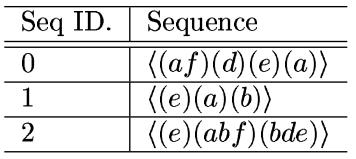
\includegraphics[width=0.4\linewidth]{D}}\caption*{Example}
\end{figure}
\begin{itemize}
\item $D_{\langle (\alpha f) \rangle} = \{ \langle (d)(e)(\alpha) \rangle, \langle (bde) \rangle \}$
\item $D_{\langle (e)(\alpha) \rangle} = \{ \$,\langle (b) \rangle,\langle (\_bf)(bde) \rangle \}$
\end{itemize}
\end{frame}

\begin{frame}{Lexicographic Sequence Tree}{{\it Set Lexicographic Order}}
\begin{itemize}
\item Let $t = \{ i_1,i_2,...,i_k\}, t'=\{j_1,j_2,...,j_l\}$, where $i_1 \leq ... \leq i_k$ and $j_1 \leq ... \leq j_l$
\item $t < t'$ iff {\it either} of the following is true:
\begin{enumerate}
\item $0 \leq h \leq min\{k,l\}$, we have $i_r = j_r$ for $r < h$, and $i_h < j_h$
\item $k < l$, and $i_1 = j_1,i_2 = j_2,...,i_k=j_k$
\end{enumerate}
\end{itemize}
Example: $(a,f) < (b,f), (a,b) < (a,b,c)$ and $(a,b,c) < (b,c)$
\end{frame}

\begin{frame}{Lexicographic Sequence Tree}{{\it Sequence Lexicographic Order}}
\begin{enumerate}[i]
\item if $s' = s \diamond p$, then $s < s'$
\item if $s = \alpha \diamond_i p$ and $s' = \alpha \diamond_s p'$, no matter what is order relation between $p$ and $p'$ is, $s < s'$
\item if $ s = \alpha \diamond_i p$ and $s' = \alpha \diamond_i p',~p < p'$ indicated $s < s'$
\item $s = \alpha \diamond_s p$ and $s' = \alpha \diamond_s p',~p < p'$ indicates $s < s'$
\end{enumerate}
Example: $\langle (a,b) \rangle < \langle (a,b)(a) \rangle$; $\langle (a,b) \rangle < \langle (a)(a) \rangle$
\end{frame}

\begin{frame}{Lexicographic Sequence Tree}{{\it Lexicographic Sequence Tree} construction}
\begin{enumerate}
\item each node in the tree corresponds to a sequence, and the root is a {\it null} sequence;
\item if a parent node corresponds to a sequence {\it s}, its child is either an itemset-extension of {\it s}, or a sequence-extension of {\it s};
\item the left sibling is less than the right sibling in sequence lexicographic order.
\end{enumerate}
\end{frame}

\begin{frame}{Lexicographic Sequence Tree}{Lexicographic Sequence Tree and Prefix Search Tree}
\center{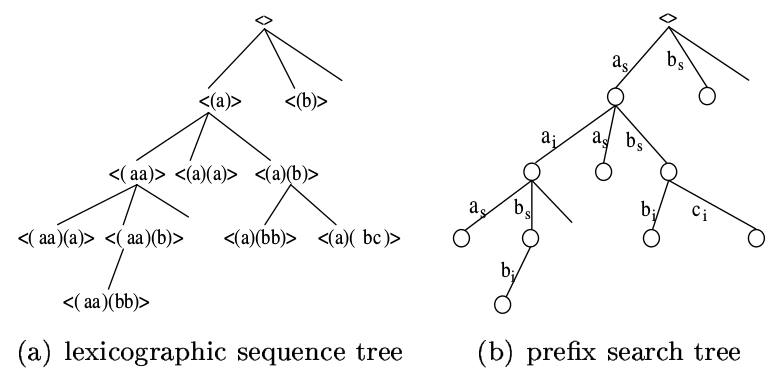
\includegraphics[width=1.\linewidth]{sequence-tree}}
\end{frame}

\begin{frame}{Lexicographic Sequence Tree}{Example}\label{D-sample}
\begin{figure}
\center{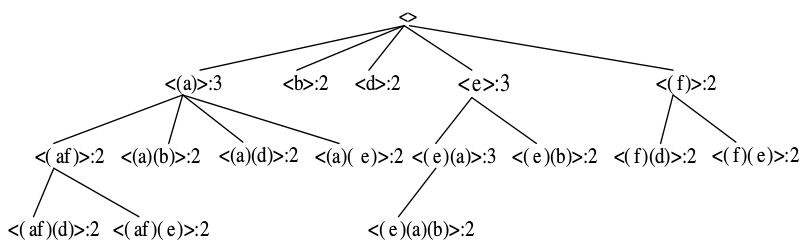
\includegraphics[width=1.\linewidth]{sequence-tree-sup}}\caption*{Lexicographic Sequence Tree with min\_sup = 2}
\end{figure}
\center{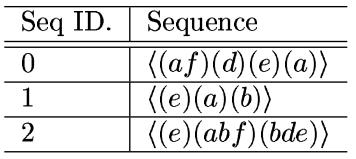
\includegraphics[width=0.4\linewidth]{D}}
\end{frame}

\begin{frame}{Search Space Pruning and Prefix Sequence Lattice}{LEMMA 1 (Common Prefix)}
LEMMA 1. {\it Given a subsequence s, and its projected database $D_s$, if $\exists\alpha$, $\alpha$ is a common prefix for all the sequences with the same extension type (either itemset or sequence - extension) in $D_s$, then $\forall\beta$, if $s \diamond \beta$ is closed, $\alpha$ must be a prefix of $\beta$. That means $\forall\beta \sqsubset \alpha$, we need not search $s \diamond \beta$ and its descendants except the branch of $s \diamond \alpha$.}\\
\splitline
{\bf Example:} $D_s = \{ \langle (d)(e)(af) \rangle, \langle (d)(e)(fg) \rangle \}$, all the sequences in $D_s$ share a common prefix $\alpha = \langle (d)(e) \rangle$, so any sequence with prefix {\it s} but not $s \diamond \langle (d)(e) \rangle$ must not be closed. So we can ``jump'' to the branch $s \diamond \alpha$.
\end{frame}

\begin{frame}{Search Space Pruning and Prefix Sequence Lattice}{LEMMA 2 (Partial Order)}
LEMMA 2. {\it Given a sequence s, and its projected database $D_s$, if among all the sequences in $D_s$, and item $\alpha$ does always occur before an item $\beta$ (either in the same itemset for all sequences in $D_s$ or in a different itemset, but not both), then $D_{s\diamond\alpha\diamond\beta} = D_{s\diamond\beta}$. Therefore, $\forall\gamma,s\diamond\beta\diamond\gamma$ is not closed. We need not search any sequence in the branch of $s \diamond \beta$.}\\
\end{frame}

\begin{frame}{Search Space Pruning and Prefix Sequence Lattice}{Theorem 1 (Equivalence of Projected Databases)}
\begin{itemize}
	\item $\mathcal{I}(D) = \sum\limits_{i=1}^n l(s_i)$: total number items in D
\end{itemize}
{\it Theorem 1:} Given 2 sequences, $s,~s',~s \sqsubseteq s'$, then $$D_s = D_{s'} \Leftrightarrow \mathcal{I}(D_s) = \mathcal{I}(D_{s'})$$\\
{\it Example:} Consider D-sample on \ref{D-sample} slide.
\begin{itemize}
\item $D_{\langle (af) \rangle} = D_{\langle (f) \rangle} = \{ \langle (d)(e) \rangle,\langle (de) \rangle \}$, and
\item  $\mathcal{I}(D_{ \langle (af) \rangle }) = \mathcal{I}(D_{\langle (f) \rangle}) = 4$.
\end{itemize}
Based on Theorem 1, the following search space pruning can be achieved.
\end{frame}

\begin{frame}{Search Space Pruning and Prefix Sequence Lattice}{{\it Proof} of Theorem 1}
\begin{itemize}
\item $D_s = D_{s'} \rightarrow \mathcal{I}(D_s) = \mathcal{I}(D_{s'})$ (obvious);
\item Since $s \sqsubseteq s'$, then $D_{s'} \sqsubseteq D_s$ and $\mathcal{I}(D_{s'}) \leq \mathcal{I}(D_s)$;
\item {\it The equality} between  $\mathcal{I}(D_{s'})$ and $\mathcal{I}(D_s)$ holds only if $\forall\gamma \in D_{s'}$, $\gamma \in D_s$, and vice versa. {\bf Therefore}, $D_s = D_{s'}$.
\end{itemize}
\end{frame}

\begin{frame}{Search Space Pruning and Prefix Sequence Lattice}{LEMMA 3 (Early Termination by Equivalence)}
LEMMA 3. {\it Given 2 sequences, $s \sqsubseteq s'$ and also $\mathcal{I}(D_s) = \mathcal{I}(D_{s'})$, then $\forall\gamma, support(s \diamond \gamma) = support(s' \diamond \gamma)$.}\\
\splitline
{\bf Example:} Consider D-sample on \ref{D-sample} slide.
\begin{itemize}
\item $\mathcal{I}(D_{\langle (af) \rangle}) = \mathcal{I}(D_{\langle (f) \rangle})$;
\item both $\langle ((af)(d)) \rangle$ and $\langle (af)(e) \rangle$ are frequent;
\end{itemize}
We can conclude that the support of $\langle (af)(d) \rangle$ and $\langle (f)(d) \rangle$, $\langle (af)(e) \rangle$ and $\langle (f)(e) \rangle$ are the same without knowing the support of $\langle (f)(e) \rangle$ and $\langle (f)(d) \rangle$.
\end{frame}

\begin{frame}{Search Space Pruning and Prefix Sequence Lattice}{Projected database closed set (LS)}
\begin{itemize}
\item $LS = \{s | support(s) \geq min\_sup \}$ and $\nexists s'$, s.t $s \sqsubseteq s'$ and  $\mathcal{I}(D_s) = \mathcal{I}(D_{s'})$;
\item $CS \subseteq LS \subseteq FS$: instead of mining CS directly, CloSpan algorithm first produces the complete set of {\it LS}
\item then non-closed sequence elimination is applied in  {\it LS} to generate {\it CS} based of Lemma 3.
\end{itemize}
\end{frame}

\begin{frame}{Search Space Pruning and Prefix Sequence Lattice}{Corollary 1 (Backward Sub-Pattern)}
Corollary 1. {\it If a sequence s < s' and $s \sqsupset s'$, the condition of $\mathcal{I}(D_s) = \mathcal{I}(D_{s'})$ is sufficient to stop searching any descendant of $s'$ in the prefix searching tree.}
\begin{figure}
\center{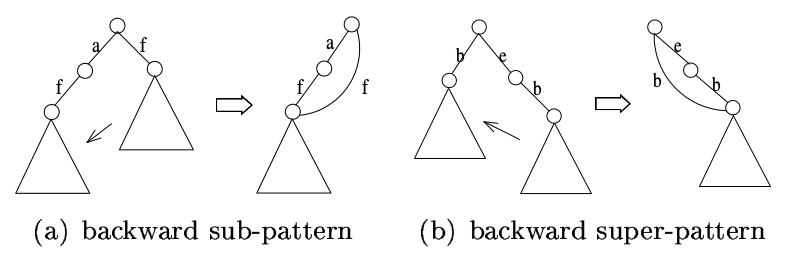
\includegraphics[width=0.6\linewidth]{backward-pattern}}
\caption*{$s'$ is {\it backward sub-pattern} of s if $s < s'$ and $s \sqsupset s'$ ($s'$ is discovered after s)}
\end{figure}
{\bf Example:} $\mathcal{I}(D_{\langle (f) \rangle}) = \mathcal{I}(D_{\langle (af) \rangle}) \rightarrow D_{\langle (f) \rangle} = D_{\langle (af) \rangle}$
\end{frame}

\begin{frame}{Search Space Pruning and Prefix Sequence Lattice}{Corollary 2 (Backward Super-Pattern)}
Corollary 2. {\it If a sequence $s < s'$ and $s \sqsupset s'$, if the condition of $\mathcal{I}(D_s) = \mathcal{I}(D_{s'})$ holds, it is sufficient to translating the descendants of s to $s'$ instead of searching any descendant of $s'$ in the prefix search tree.}\\
\splitline
{\bf Example:} the same logic as in the previous example.
\end{frame}

\begin{frame}{CloSpan: Design and Implementation}{2 main steps}
CloSpan divides mining process into 2 stages.
\begin{enumerate}
\item Generated the {\it LS} set, a superset of closed frequent sequences, and stores it in a prefix sequence lattice;
\item it does post-pruning to eliminate non-closed sequences.
\end{enumerate}
\end{frame}

\begin{frame}{CloSpan: Design and Implementation}{Algorithm 1: ClosedMining({\it D, min\_sup, L})}
\begin{figure}
\center{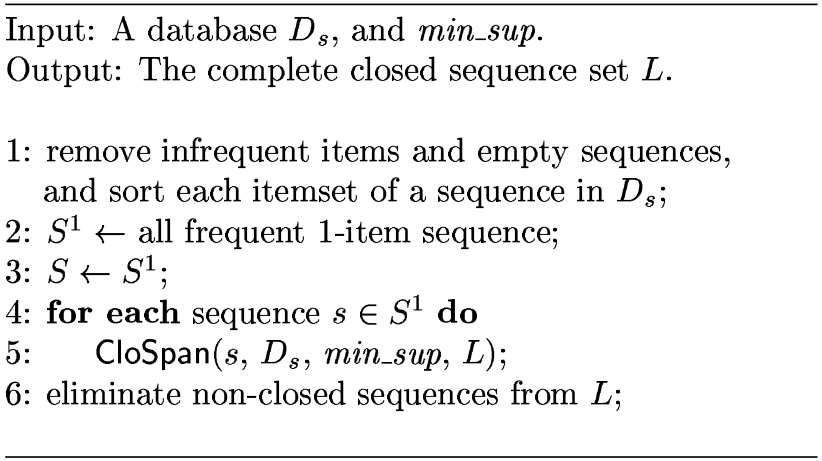
\includegraphics[width=0.8\linewidth]{ClosedMining}}
\end{figure}
\end{frame}

\begin{frame}{CloSpan: Design and Implementation}{Algorithm 2: CloSpan({\it s, $D_s$, min\_sup, L})}
\begin{figure}
\center{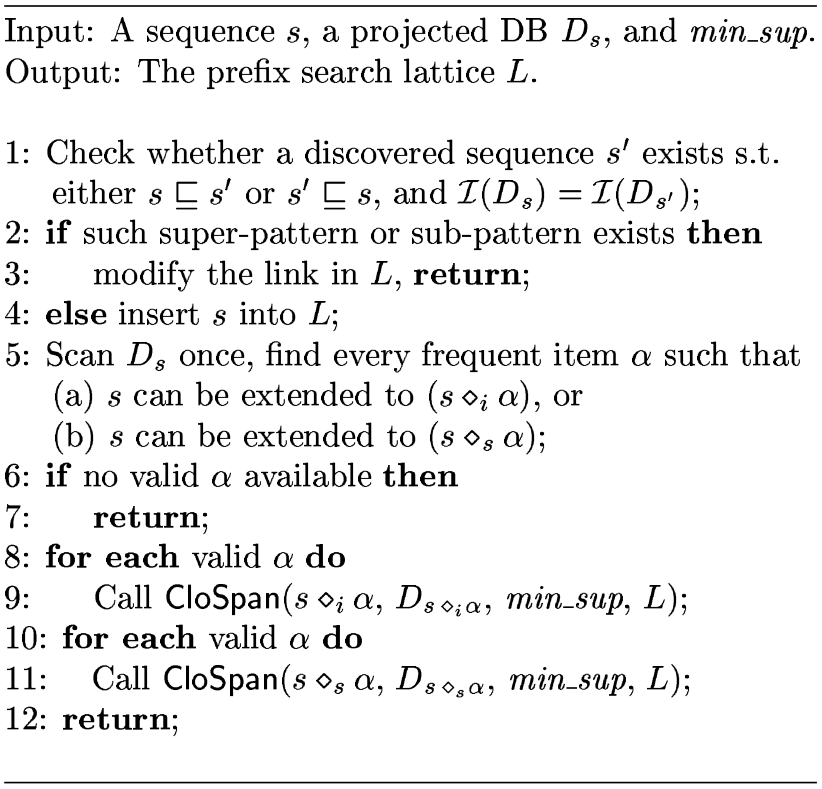
\includegraphics[width=0.6\linewidth]{CloSpan}}
\end{figure}
\end{frame}

\begin{frame}{CloSpan: Design and Implementation}{Algorithm : CloSpan}
\begin{itemize}
\item Hash index on the size of projected database in order to speed up check on Theorem 1 (1-4 lines of CloSpan);
\item if $\mathcal{I}(D_{s'}) = \mathcal{I}(D_s)$ then;
\item if $s \sqsubseteq s'$, then we do not add $\langle \mathcal{I}(D_s),s \rangle$;
\item if $s' \sqsubseteq s$, then we replace $\langle \mathcal{I}(D_{s'}),s' \rangle$ with $\langle \mathcal{I}(D_s),s \rangle$.
\end{itemize}
\begin{figure}
\center{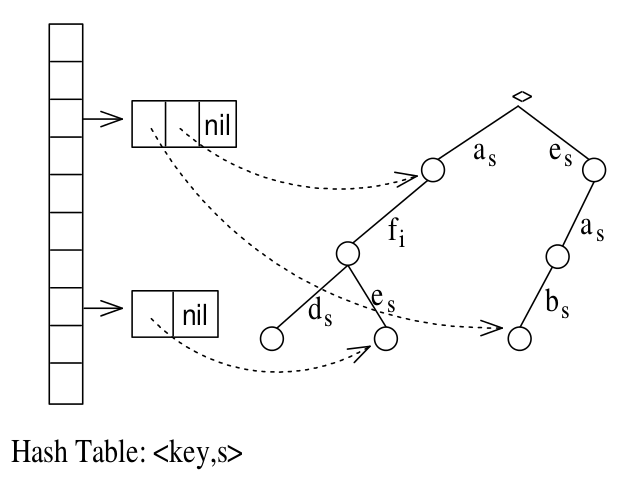
\includegraphics[width=0.4\linewidth]{HashTable}}
\caption*{$\langle \mathcal{I}(D_s),s \rangle$}
\end{figure}
\end{frame}

\begin{frame}{CloSpan: Design and Implementation}{Algorithm 3: checkProjectedDBSize({\it s, k, H})}
Corresponds to line 1-4 in Algorithm 2.
\begin{figure}
\center{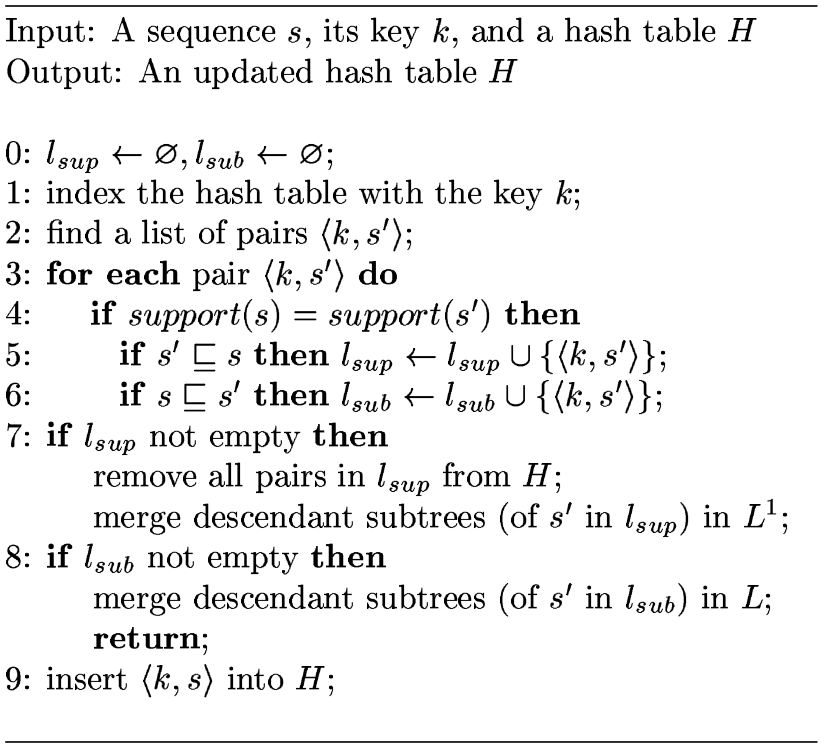
\includegraphics[width=0.6\linewidth]{checkProjectedDBSize}}
\end{figure}
\end{frame}

\begin{frame}{CloSpan: Design and Implementation}{Algorithm 3: hash function algorithm}
\begin{itemize}
\item Database size range from 0 to $\mathcal{I}(D)$, so if the values of $\mathcal{I}(D_s)$ are dense in a small range, performance degrade;
\item by Theorem 1 we could use necessary propositions of holding $D_s = D_{s'}$ in a part of hash key;
\item $\mathcal{L}(D_s) = \mathcal{I}(D_s) + \sum^{m}_{j=1} \sum^{n}_{k=i_j+1}l(s_k)$;
\item if $s \sqsupseteq s'$, $\mathcal{L}(D_s) = \mathcal{L}(D_{s'}) \leftrightarrow \mathcal{I}(D_s) = \mathcal{I}(D_{s'})$.
\end{itemize}
\end{frame}

\begin{frame}{Non-Closed Sequence Elimination}{Check out for super sequence}
\begin{itemize}
\item $support(s)$ as its Hash function 
\item find all the sequences with the same support of s
\item check whether there is a super-sequence containing s.
\item if $s \sqsupseteq s'$ and $support(s) = support(s') \rightarrow \mathcal{T}(D_s) = \mathcal{T}(D_{s'})$ (corresponding sequences' id sum)
\item that's why $\mathcal{T}(D_s) = \mathcal{T}(D_{s'})$ could be used as a Hash function instead of support (more sparse)
\end{itemize}
\end{frame}

\begin{frame}{Conclusion}{{\it CloSpan}}
\begin{itemize}
\item Solve closed sequential pattern mining problem;
\item {\it CloSpan} outperforms {\it PrefixSpan} by more than one order of magnitude;
\item capable of mining longer frequent sequences in a large data set with low min\_sup;
\item it does not modify the frequent pattern mining algorithm: it only defines the early termination condition of search branch;
\item this method can be extended to other existing sequential pattern mining algorithms (SPADE, SPAM).
\end{itemize}
\end{frame}

\begin{frame}{Possible improvements}{{\it CloSpan}}
\begin{itemize}
\item The performance of CloSpan is achieved by smart prunning method, do it more smart;
\item Do not need to keep track of any single historical frequent closed sequence (or candidate) for a new pattern’s closure checking.
\end{itemize}
\end{frame}

\begin{frame}{Possible improvements}{{\it BIDE algorithm}}
\begin{enumerate}
\item BIDE consumes much less memory and can be an order of magnitude faster than CloSpan when the support is low;
\item BIDE has linear scalability against base size in terms of runtime efficiency and space usage;
\item the BackScan pruning method is very effective in enhancing the performance of BIDE.
\end{enumerate}
\end{frame}

\begin{frame}{CloSpam in trajectory Mining}{Sequential Pattern Mining from Trajectory Data}
\begin{itemize}
  \item need more studies: IPCA and DBScan on Trajectory data.
  \item CloSpan could be used as unsupevised algorithm for detecting most crowded paths in a city.
  \item ...
\end{itemize}
\end{frame}

\end{document}